\section{Typical deviations}
\marginpar{\red{Lecture 4}}

In the previous section we have seen that the mean \(\mean{X}_n =
\frac1n\sum_{k=1}^n X_k\) converges to the expected value \(\E{X}\).
Consequently the deviations from the mean converge to zero. From Bienaymé (Lemma
\ref{lem: Bienaymé}) we discovered for uncorrelated identically distributed
random variables
\[
    \var{\mean{X}_n} = \tfrac1n \var{X_1}.
\]
Since the variance is a squared measure of deviation, this means
that the typical size of the deviation of the mean \(\mean{X}_n\) from the expectation
\(\E{X}\) is of order \(\frac1{\sqrt{n}}\).
Specifically the rescaled mean \(\sqrt{n}\,\mean{X}_n\) has
constant variance
\[
    \var{\sqrt{n}\,\mean{X}_n} = \var{X_1},
\]
and consequently by Chebyshev's inequality the deviation probability of order \(\frac{1}{\sqrt{n}}\) is
bounded by a constant
\[
    \prob[\Big]{\norm{\mean{X}_n - \E{X}} > \frac{\epsilon}{\sqrt{n}}}
    \le \frac{\var{X_1}}{\epsilon^2}.
\]
Of course this bound may be very loose but we will find that this is indeed
the size of typical deviations. Moreover the ``Central Limit Theorem''
characterizes the frequency of these typical deviations. Specifically, the asymptotic distribution of \(\sqrt{n}\,
\mean{X}_n\) is the normal distribution. Of course since the distribution of
\(\sqrt{n}\, \mean{X}_n\) is centered at \(\E{\sqrt{n}\, \mean{X}_n} = \sqrt{n}
\E{X}\) it is necessary to consider centered random variables \(X_n -
\E{X_n}\).


\subsection{Moment generating functions}
\label{sec: moment generating functions}

We start with a sketch of the argument why special ``Moment generating
functions'' will help us with the asymptotic distribution of sums.

Observe that the exponential function converts sums into products and the
expectation of independent products factorizes, thus for \(X_1,\dots, X_n\)
independent, identically distributed real random variables
\[
    \E[\Big]{\exp\Bigl(t\sum_{i=1}^n X_i\Bigr)} = \E[\Big]{\prod_{i=1}^n \exp(tX_i)}
    \overset{\text{indep.}}= \prod_{i=1}^n \E{\exp(tX_i)}
    = \E{\exp(tX_1)}^n
\]
The strategy is now essentially the following: Define the special function
\(\MGF_{X_1}(t) = \E{\exp(t X_1)}\) and observe that
by the equation above we have
\begin{equation}
    \label{eq: means and moment generating functions}    
    \MGF_{\sqrt{n} \bar{X}_n}(t) = \MGF_{X_1}(\tfrac{t}{\sqrt{n}})^n.
\end{equation}
If this function \(\MGF_{X_1}\) characterizes the distribution of \(X_1\) like a
distribution function and the above converges in \(n\), then we obtain the
limiting distribution of \(\sqrt{n}\,\mean{X}_n\). The reason \eqref{eq: means
and moment generating functions} would converge in \(n\) is that
\begin{enumerate}[label=\textbf{Step \arabic*:},itemindent=2em]
    \item \(\frac{t}{\sqrt{n}}\) converges to \(0\) so the Taylor approximation
    of \(\MGF_{X_1}\) becomes asymptotically accurate 
    \item the Taylor coefficients of \(\MGF_{X_1}\) will be exactly the moments
    \(\E{X_1^k}\) (Lemma \ref{lem: moment generating function representation}), consequently
    \[
        \MGF_{X_1}(t) = \underbrace{\E{X^0}}_{=1} + \underbrace{\E{X^1}}_{=0} t + \underbrace{\E{X^2}}_{\sigma^2} \frac{t^2}{2} + \dots
    \]
    \item the last step is an application of \((1+\frac{x}n)^n \to e^x\) (the
    compound interest formula -- Lemma \ref{lem: compound interest}) to get
    \[
        \MGF_{X_1}(\tfrac{t}{\sqrt{n}})^n
        = (1 + \tfrac{\sigma^2 t^2}{2n} + \dots)^n \to \exp(\tfrac{\sigma^2 t^2}2).
    \]
\end{enumerate}
A wrinkle in this strategy is that \(\E{\exp(tX_1)}\) may be infinite. The
solution to this problem is to consider complex \(t\).

Let us now build up the arguments properly. We start by
defining ``Moment generating functions''.

\begin{definition}[Moment generating functions]
    The ``Moment generating function'' of a random variable \(X\) in 
    \(\real^\dims\) is given by
    \[
        \MGF_X(t) \coloneq \E{\exp(\scp{t, X})}
        \qquad t\in \complex^\dims.
    \]
    The ``characteristic function'' is given by
    \[
        \charFct_X(t) \coloneq \MGF_X(i t) = \E{\exp(i\scp{t,X})}
        \qquad t\in \real^\dims.
    \]
    Outside the field of probability theory one typically uses \(-t\) 
    instead of \(t\), and 
    \begin{itemize}[noitemsep]
        \item \(\mathcal{L}\set{\Pr_X}(t) = \MGF_X(-t)\) is the ``Laplace
        transform'',
        \item \(\mathcal{F}\set{\Pr_X}(t) = \charFct_X(-2\pi t)\) is the ``Fourier
        transform''. 
    \end{itemize}
\end{definition}

As mentioned in the introduction, \(\MGF_X\) is called the ``Moment
generating function'' because its Taylor coefficients are the moments.
For simplicity we restrict ourselves to real valued random variables
in the following (see Exercise \ref{ex: multivariate moment generating function}
for the general case).

\begin{lemma}[Moment generating function representation]
    \label{lem: moment generating function representation}
    Let \(X\) be a real valued random variable with \(\MGF_{X}(r) < \infty\) and
    \(\MGF_{X}(-r) < \infty\) for for some real \(r>0\). Then all moments exist,
    that is \(\E{\abs{X}^n} <\infty\) for all \(n\), and \(\MGF_X\) is
    analytic (finite) on the ball with radius \(r\) with the representation
    \[
        \MGF_X(t) = \sum_{k=0}^\infty \E{X^k}\frac{t^k}{k!} \qquad \forall t\in \complex, |t| \le r.
    \]
    in particular this implies \(\frac{d^n}{dt^n} \MGF_X(0) = \E{X^n}\).
\end{lemma}
\begin{proof}
    For the finiteness of all moments observe that
    \[
        \abs{x}^n
        \le \tfrac{n!}{r^n} e^{r\abs{x}}
        \le \tfrac{n!}{r^n} \bigl(e^{r x} + e^{-r x}\bigr)
    \]
    implies
    \[
        \E{\abs{X}^n} \le \tfrac{n!}{r^n} \bigl(\MGF_X(r) + \MGF_X(-r)\bigr) < \infty.
    \]
    Now for the representations, we have for all \(t\in \complex, |t| \le r\)
    that
    \[\begin{aligned}
        \E[\Big]{\sum_{k=0}^\infty \frac{\abs{tX}^k}{k!}}
        = \E{e^{\abs{tX}}}
        &\le \E{e^{r\abs{X}}}
        \\
        &\le \E{e^{r X} + e^{-r X}}
        = \MGF_X(r) + \MGF_X(-r) < \infty.
    \end{aligned}
    \]
    Consequently we may apply Fubini (or the DCT to partial sums) to obtain
    \[
        \MGF_X(t)
        = \E[\Big]{\sum_{k=0}^\infty \frac{tX^k}{k!}}
        \overset{\text{Fub.}}= 
        \sum_{k=0}^\infty \E[\Big]{\frac{tX^k}{k!}}
        = \sum_{k=0}^\infty \E{X^k}\frac{t^k}{k!}.
        \qedhere
    \]
\end{proof}

While the moment generating function needs all moments to exist, the
characteristic function is always well defined since \(\abs{e^{itx}} =1\)
implies
\begin{equation}
    \label{eq: bound on characteristic function}    
    \abs{\charFct_X(t)} \le \E{\abs{e^{itX}}} = 1
    \qquad \forall t\in \real^\dims.
\end{equation}
However, if moments do exist, the characteristic function has a similar
representation.

\begin{lemma}[Characteristic function representation]
    \label{lem: characteristic function representation}
    Let \(X\) be real valued with \(\E{\abs{X}^n} < \infty\) for some
    \(n\), then \(\charFct_X\) is \(n\)-times continuously differentiable
    with
    \[
        \charFct_X(t) = \sum_{k=0}^n \E{X^k}\frac{(it)^k}{k!} + o(t^n).
    \]
    If all the moments are finite and \(\lim_{n\to \infty}
    \frac{t^n}{n!}\E{\abs{X}^n} =0\) for some \(t>0\), then
    \(\charFct_X\) is a power series with convergence radius at least \(t\).
\end{lemma}
\begin{proof}
    Let us first show that the \(n\)-th derivative exists. To this end
    observe that
    \[
        \frac{d^n}{dt^n} \exp(i t x) = (ix)^n \exp(i t x).
    \]
    Consequently, we have \(\abs{\frac{d^n}{dt^n} \exp(i t x)} \le \abs{x}^n\) such that
    \(\abs{X}^n\) is an integrable dominating function of the derivative
    by assumption that \(\E{\abs{X}^n} < \infty\). Since the
    finite-difference quotients are bounded by the derivative using the mean value
    theorem we may thus apply the Dominated Convergence Theorem (DCT) to
    interchange differentiation and expectation to obtain
    \[
        \frac{d^n}{dt^n} \charFct_X(t)
        = \E[\Big]{\frac{d^n}{dt^n} \exp(i t X)}
        = \E{(iX)^n \exp(i t X)}.
    \]
    We thus have that the characteristic function is \(n\)-times differentiable
    and the representation is the Taylor expansion around zero.
    Last assume that all moments are finite. Since the derivatives are bounded
    by the moments
    \[
        \abs{\charFct_X^{(n)}(t)} \le \E{\abs{iX}^n \abs{\exp(i t X)}} = \E{\abs{X}^n},
    \]
    the mean value remainder with \(\xi \in (0,t)\) is bounded by
    \[
        \abs{R_{n-1}(t)} = \abs[\Big]{\frac{t^{n}}{n!} \charFct_X^{(n)}(\xi)}
        \le \frac{\abs{t}^{n}}{n!} \E{\abs{X}^{n}}.
    \]
    Its convergence to zero therefore follows directly from the assumption.
\end{proof}

As we outlined in the beginning of this section the moment generating function
and characteristic function characterize the distribution of a random variable.
This is a non-trivial fact from measure theory.

\begin{fact}[Uniqueness]
    \label{fact: uniqueness of mgf and char fct}
    Let \(X, Y\) be random variables in \(\real^\dims\). Then
    \begin{align*}
        X \overset{d}= Y
        \quad &\iff\quad
        \charFct_X(t) = \charFct_Y(t)
        \quad \forall t\in \real^\dims.
        \intertext{
    If the moment generating functions \(\MGF_X\) and \(\MGF_Y\)
    are finite in a neighborhood of zero \(\ball{0}{\epsilon}\), then the following is also equivalent
        }
        \quad &\iff\quad
        \quad \MGF_X(t) = \MGF_Y(t)
        \quad \forall t\in \ball{0}{\epsilon}.
    \end{align*}
\end{fact}

More than just uniquely characterizing distributions, they also
characterize convergence in distribution. This is known as Lévy's continuity
theorem.

\begin{mdframed}[innertopmargin=0pt]%
\begin{fact}[Lévy's continuity theorem]
    \label{fact: levy continuity}
    Let \((X_n)_{n\in \nat}\) and \(X\) be random variables in \(\real^\dims\) then
    the following are equivalent:
    \begin{enumerate}[label=(\roman*),noitemsep]
        \item\label{it: Lévy's cont d} \(X_n \overset{d}\to X\),
        \item\label{it: Lévy's cont char} \(\charFct_{X_n}(t) \to \charFct(t)\) for all \(t\in \real^\dims\).
    \end{enumerate}
    Moreover, \(\charFct_{X_n}(t) \to f(t)\) for all \(t\in \real^\dims\) and \(f\) continuous at
    \(0\) implies the existence of a random variable \(X\) with
    \(\charFct_X(t) = f(t)\).
\end{fact}
\end{mdframed}

\begin{remark}[Moment generating functions]
    Convergence of the moment generating functions similarly implies convergence
    in distribution if the moment generating functions are finite in a
    neighborhood of zero \citep{curtissNoteTheoryMoment1942}.
    However in practice the characteristic function is preferred 
    since it is always finite.
\end{remark}
\begin{remark}[Infinite dimensions]
    Lévy's continuity theorem does not hold in
    infinite dimensions and can therefore not be generalized to hilbert spaces
    (Exercise \ref{ex: counterexample levy's continuity in infinite dim}).
\end{remark}

\begin{proof}[Proofsketch (Lévy's continuity theorem)]
    ``\ref{it: Lévy's cont d} \(\Rightarrow\) \ref{it: Lévy's cont char}''
    follows from Euler's formula \(\exp(i\scp{t, x}) = \cos(\scp{t, x}) + i \sin(\scp{t, x})\) since both \(\cos\) and \(\sin\) 
    are bounded and continuous functions and thus by \ref{it: b.cont}
    \begin{equation}
        \label{eq: char function convergence}    
        \charFct_{X_n}(t)
        = \E{\exp(i\scp{t, X_n})}
        \to \E{\exp(i\scp{t, X})}
        = \charFct_X(t).
    \end{equation}
    ``\ref{it: Lévy's cont d} \(\Rightarrow\) \ref{it: Lévy's cont char}'' is significantly
    more difficult and requires the concept of ``separating function classes''
    see e.g.
    \citep{klenkeProbabilityTheoryComprehensive2014,kallenbergFoundationsModernProbability2002}.
\end{proof}

We can now prove the Cramér-Wold part of the joint convergence theorem (Theorem
\ref{thm: joint convergence}) as a corollary of Lévy's continuity theorem.
This result is extremely useful in lifting univariate convergence results to
multivariate results.

\begin{corollary}[Cramér-Wold]
    \label{cor: cramer wold}
    Let \((X_n)_{n\in \nat}\) and \(X\) be random variables in \(\real^\dims\). Then
    \[
        \scp{t, X_n} \overset{d}\to \scp{t, X} \quad \forall t \in \real^\dims
        \quad \iff \quad
        X_n \overset{d}\to X.
    \]
\end{corollary}
\begin{proof}
    ``\(\Leftarrow\)'' follows from continuous mapping as the inner product
    is continuous. For ``\(\Rightarrow\)'' we observe that the assumption
    implies \eqref{eq: char function convergence},
    which means that the characteristic functions converges for all
    \(t\) and thus \(X_n \overset{d}\to X\) by Lévy's continuity theorem.
\end{proof}

\subsection{The central limit theorem}

\begin{wrapfigure}[6]{o}{0.35\textwidth}
    \vspace{-2em}
    \scalebox{0.7}{
    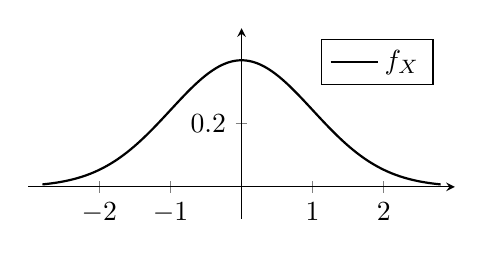
\begin{tikzpicture}
    \begin{axis}[
        axis lines=middle,
        xmin=-3, xmax=3,
        ymin=-0.1, ymax=0.5,
        samples=200,
        domain=-2.8:2.8,
        width=7cm,
        height=4cm,
        xtick={-2, -1, 0, 1, 2},
        ytick={0.2},
        yticklabels={0.2},
        legend style={at={(0.95,.7)}, anchor=south east},
    ]

    % density
    \addplot[thick] {
        exp(-x^2/2)/(sqrt(2*pi))
    };
    \addlegendentry{$f_X$}
    \end{axis}
\end{tikzpicture}
    }
    \caption{Standard normal density \(\density_X\) from \eqref{eq: standard normal density}}
\end{wrapfigure} 
We will now characterize the asymptotic distribution of the rescaled mean using
Lévy's continuity theorem. With the benefit of historical hindsight we already
know that the limiting distribution is the normal distribution so we start
with its definition and the calculation of its characteristic function.

\begin{definition}[Univariate normal distribution]
    \label{def: univariate normal distribution}
    A random variable \(X\) in \(\real\) is \textbf{standard normal
    distributed} if it has density
    \begin{equation}
        \label{eq: standard normal density}
        \density_X(x)
        = \frac1{\sqrt{2\pi}}
        \exp\bigl(-\tfrac{x^2}{2}\bigr).
    \end{equation}
    A random variable \(X\) in \(\real\) is \textbf{normal
    distributed} with mean \(\mu \in \real\) and variance \(\sigma^2 \mathop{\red{\ge}} 0\),
    denoted \(X \sim \normal{\mu, \sigma^2}\), if one of the following
    equivalent conditions holds:
    \begin{enumerate}[label=(\roman*)]
        \item\label{it: standard normal} \(X \overset{d}= \mu + \sigma Y\) where \(Y\) is a \underline{standard normal} random variable,

        \item\label{it: mgf normal}
        % the moment generating function of \(X\) is given by
        \(
            \MGF_X(t)
            = \exp\bigl(\mu t + \tfrac12 \sigma^2 t^2\bigr),
        \)

        \item\label{it: char fct normal}
        %the characteristic function of \(X\) is given by
        \(
            \charFct_X(t)
            = \exp\bigl(i \mu t - \tfrac12 \sigma^2 t^2\bigr).
        \)
    \end{enumerate}
\end{definition}
\begin{remark}
    We do not require \(\sigma^2 > 0\) in the definition! However, if
    \(\sigma^2>0\), then by Exercise \ref{ex: density of normal distribution} \(X\sim \normal{\mu, \sigma^2}\) has density
    \[
        \density_X(x) = \frac1{\sqrt{2\pi \sigma^2}}
        \exp\bigl(-\tfrac{(x-\mu)^2}{2\sigma^2}\bigr).
    \]
    This is usually taken as the definition of the normal distribution. However
    this definition does not work for \(\sigma^2=0\) and would prevent the
    central limit theorem to hold in this case. And the importance of the normal
    distribution is solely justified by the CLT. Moreover the multivariate normal
    distribution will be less awkward to define if we allow zero variance.
\end{remark}
\begin{proof}[Proof (Definition \ref{def: univariate normal distribution} is well defined)]
    We delay the proof that the density \eqref{eq: standard normal density} integrates to one
    to Lemma \ref{lem: standard normal density integrates to one}. The equivalence of the definitions of the
    normal distribution follows from a calculation of the moment generating and
    characteristic functions due to the uniqueness of these functions (Fact
    \ref{fact: uniqueness of mgf and char fct}). We start with the moment
    generating function. Assuming \ref{it: standard
    normal} we have
    \begin{equation}
        \label{eq: mgf normal calculation}    
        \MGF_X(t) = \MGF_{\mu + \sigma Y}(t) = \E{e^{t(\mu + \sigma Y)}} = e^{\mu t}\MGF_Y(\sigma t)
    \end{equation}
    and thus it suffices to calculate the moment generating function \(\MGF_Y\),
    \[
        \MGF_Y(t)
        = \int_\real \exp(tx) \frac1{\sqrt{2\pi}}
        \exp\bigl(-\tfrac{x^2}{2}\bigr) dx
        = \frac1{\sqrt{2\pi}} \int_\real
        \exp\Bigl(-\frac1{2}\bigl(x^2 - 2 tx\bigr)\Bigr) dx.
    \]
    The exponent may be brought into the form \((x-\tilde{\mu})^2 +
    c\), where the residual \(c\) is constant in \(x\).
    Specifically, we have
    \[
        x^2 - 2 tx
        = \bigl(x^2 - 2 t x + t^2 - t^2\bigr)
        = (x - t)^2 - t^2.
    \]
    Put back into the integral this yields
    \[
        \MGF_Y(t)
        = \exp\bigl(\tfrac12 t^2\bigr)
        \frac1{\sqrt{2\pi}} \int_\real
        \exp\bigl(-\tfrac1{2}(x - t)^2\bigr) dx
        = \exp\bigl(\tfrac12 t^2\bigr),
    \]
    and consequently by \eqref{eq: mgf normal calculation} \(\MGF_X(t) = e^{\mu t} e^{\frac12 \sigma^2 t^2}\).
    For the characteristic function observe that \(t\mapsto e^{\mu t + \frac12
    \sigma^2 t^2}\) is an entire analytic function on \(\complex\), it is the
    unique analytic continuation of \(\MGF_X\) to \(\complex\) and thus
    \(\charFct_X(t) = \MGF_X(it) = e^{i \mu t - \frac12 \sigma^2 t^2}\).
\end{proof}

We are finally ready to prove the univariate central limit theorem.

\begin{mdframed}[innertopmargin=0pt]
\begin{theorem}[Univariate CLT]
    \label{thm: univariate central limit theorem}
    Let \((X_n)_{n\in \nat}\) be iid copies of the random variable \(X\in
    \cL^2(\real)\) with mean \(\mu = \E{X}\) and variance \(\sigma^2 =
    \var{X}\). Then
    \[
        \sqrt{n}\bigl(\mean{X}_n - \mu\bigr)
        \overset{d}\to \normal{0, \sigma^2}.
    \]
\end{theorem}
\end{mdframed}

\begin{proof}
    Without loss of generality we may assume that \(m=0\) since we can
    consider the centered random variables \(\tilde{X}_n = X_n - m\).
    We then have
    \[
        \charFct_{\sqrt{n} \mean{X}_n}(t)
        = \E[\Big]{\exp\Bigl(i \frac{t}{\sqrt{n}} \sum_{k=1}^n X_k\Bigr)}
        = \prod_{k=1}^n \E{\exp\Bigl(i \tfrac{t}{\sqrt{n}} X_k\Bigr)}
        = \charFct_{X}(\tfrac{t}{\sqrt{n}})^n.
    \]
    Since second moments are finite, \(\E{X_1} = 0\) and \(\sigma^2 =
    \E{X_1^2}\), we have by the representation for characteristic functions
    (Lemma \ref{lem: characteristic function representation})
    \[
        \charFct_X(\tfrac{t}{\sqrt{n}})
        = \Biggl[\sum_{k=0}^2 \E{X^k}\frac{(i\frac{t}{\sqrt{n}})^k}{k!} + o\Bigl(\frac{t^2}{n}\Bigr)\Biggr]
        = 1 - \frac{\sigma^2 t^2}{2 n} + o\Bigl(\frac{t^2}{n}\Bigr).
    \]
    Consequently we have by Lemma \ref{lem: compound interest}
    \[
        \charFct_{\sqrt{n} \mean{X}_n}(t)
        = \Bigl(1 - \tfrac{\sigma^2 t^2}{2 n} + o(\tfrac{t^2}{n})\Bigr)^n
        \to e^{-\frac12 \sigma^2 t^2}.
    \]
    Since that is the characteristic function of a normal distribution
    with mean zero and variance \(\sigma^2\) (Definition \ref{def: univariate
    normal distribution}) the claim follows by Lévy's continuity theorem (Fact \ref{fact: levy continuity}).
\end{proof}

In the proof of the central limit theorem we used the compound interest
formula in the complex case. This is the following Lemma.

\begin{lemma}[Compound interest]
    \label{lem: compound interest} Let \((x_n)_{n\in \nat}\) be a sequence in \(\complex\)
    with \(x_n \to x\in \complex\). Then
    \[
        \lim_{n\to\infty} (1+\tfrac{x_n}n)^n = e^{x}.
    \]
\end{lemma}
\begin{proof}
    Note that \(\exp\) is injective on the domain \(B\coloneq\set{x+iy\in \complex: \abs{y} < \pi}\)
    with range \(\complex\setminus \real_{\le 0}\). Since \(1+\frac{x_n}n \to
    1\) this term eventually enters \(\complex\setminus \real_{\le
    0}\). Using the (analytic) inverse \(\ln\) of \(\exp\) restricted to \(B\)
    we thus have for sufficiently large \(n\)
    \[
        (1 + \tfrac{x_n}n)^n
        = \exp\bigl(\ln(1 + \tfrac{x_n}n)\bigr)^n
        = \exp\bigl(n \ln(1 + \tfrac{x_n}n)\bigr)
        = \exp\Bigl(x_n \frac{\ln(1 + \tfrac{x_n}n)}{x_n/n}\Bigr).
    \]
    \vspace*{-2ex}
    \begin{mdframed}[innertopmargin=0pt,innerbottommargin=0pt,rightline=false,topline=false,bottomline=false]
    Here we have tacitly assumed that \(x_n \neq 0\). We may
    do this without loss of generality:
    If there are only finitely many \(n\) with \(x_n=0\), then
    simply pick \(n\) large enough. In the other case
    the subsequence \((x_{n_k})_{k\in \nat}\) with \(x_{n_k} = 0\) still
    converges to \(x\) and consequently \(x=0\). In this case
    we also have \(\exp(n \ln(1+x_{n_k})) = \exp(0)= \exp(x)\) so
    we have convergence for this subsequence. We therefore only need
    to prove convergence for the remaining \(x_n\).
    Thus \(x_n\neq 0\) without loss of generality.
    \end{mdframed}
    Due to continuity it is sufficient to prove \(\frac1\lambda\ln(1 +
    \lambda) \to 1\) as \(\lambda \to 0\), where we choose \(\lambda = \frac{x_n}n\). Since the logarithm is analytic
    (complex differentiable)
    at \(1\) we however have
    \[
        \lim_{\lambda \to 0} \frac{\ln(1 + \lambda)}{\lambda}
        = \lim_{\lambda \to 0} \frac{\ln(1 + \lambda) - \ln(1)}{\lambda}
        = \ln'(1)
        = 1. \qedhere
    \]
\end{proof}

Since the normal distribution is the limit of sums, it is natural that the
distribution is stable under addition.

\begin{lemma}[Sum stability of normal distribution]
    \label{lem: sum stability of normal distribution}
    Let \(X_1,\dots, X_n\) be independent, normal random variables with \(X_i
    \sim \normal{\mu_i, \sigma_i^2}\). Then
    \[
        S_n \coloneq \sum_{i=1}^n X_i \sim \normal[\bigg]{\sum_{i=1}^n \mu_i,\; \sum_{i=1}^n \sigma_i^2}.
    \]
\end{lemma}
\begin{proof}
    We simply calculate the moment generating function using independence:
    \[\begin{aligned}[b]
        \MGF_{S_n}(t)
        &= \E[\Big]{\exp\Bigl(t \sum_{i=1}^n X_i\Bigr)}
        \overset{\text{indep.}}= \prod_{i=1}^n \MGF_{X_i}(t)
        = \prod_{i=1}^n \exp\bigl(\mu_i t + \tfrac12 \sigma_i^2 t^2\bigr)
        \\
        &= \exp\Bigl(t \sum_{i=1}^n \mu_i + \tfrac12 t^2 \sum_{i=1}^n \sigma_i^2\Bigr).
    \end{aligned}
    \qedhere
    \]
\end{proof}

\begin{remark}[Infinitely divisible distributions]
    Let \(X_1, X_2, \dots\) be iid random variables.  If the distribution of the
    sum is the same as an individual summand \(X_i\) up to location and scaling,
    that is
    \[
        X_1 + \dots + X_n \overset{d} = a_n X_1 + b_n,
    \]
    then the distribution of \(X_i\) is called \textbf{stable}. Since 
    the limit in \(n\) must still have this distribution, the CLT means that the
    normal distribution is the \emph{only} distribution with finite variance
    that has this property with \(a_n = n^{1/2}\). Fact: Without loss of generality the scaling can
    always be chosen to be of the form \(a_n = n^{1/\alpha}\) \citep[Thm.~16.22]{klenkeProbabilityTheoryComprehensive2014}.
    And for every \(\alpha\in (0, 2]\) there is exactly one stable distribution,
    the \(\alpha\)-stable distribution. The normal distribution is thus the
    only \(2\)-stable distribution. For \(\alpha\in (0,2)\) the tails
    decay according to a power law, roughly
    \[
        \prob{\abs{X} >t} \sim t^{-\alpha} \qquad t\to \infty.
    \]
    Any distribution that is the limit of rescaled iid sums must be
    \(\alpha\)-stable. This can be seen by grouping the summands into \(n\)
    block of increasing size and observing that each block converges. Thus the
    sum of blocks has the same distribution as the original sum up to location
    and scale. A different name for \(\alpha\)-stable distributions are the
    ``infinitely divisible distributions'' since they can always be written as
    the sum of an arbitrary number of iid random variables. Being the limit of
    sums and being stable are thus equivalent concepts.
\end{remark}

\subsection{The multivariate central limit theorem}
\marginpar{\red{Lecture 5}}

For the multivariate central limit theorem we need to introduce the multivariate
normal distribution. To do so we require the concept of covariance matrices.

\begin{definition}[Covariance matrix]
    Let \(X, Y\) be random variables in \(\real^\dims\) with finite second moments.
    The \textbf{mixed covariance matrix} of \(X\) and \(Y\) is given by
    \[
        \Cov{X;Y}
        = \E[\Big]{\bigl(X - \E{X}\bigr)\bigl(Y - \E{Y}\bigr)^\top}
        \in \real^{\dims \times \dims}.
    \]
    Recall that the expectation is applied entrywise (Remark \ref{rem: expectation in multiple dimensions}).
    We write \(\Cov{X} \coloneq \Cov{X;X}\) for the \textbf{covariance matrix} of \(X\).
\end{definition}
\begin{remark}[Exercise \ref{ex: covariance matrix}]
    The covariance defined in Definition \ref{def: covariance and variance
    definition} is the trace of this covariance matrix, that is \(\tr\Cov{X;Y} =
    \cov{X}{Y}\) and the mixed covariance matrix is simply a corner of the
    covariance matrix of the vector \((X,Y)\), that is
    \[
        \Cov{X,Y} \coloneq \Cov{(X,Y)} = \begin{pmatrix}
            \Cov{X} & \Cov{X;Y} \\
            \Cov{Y;X} & \Cov{Y}
        \end{pmatrix}.
    \]
\end{remark}

\begin{lemma}[Covariance matrices are positive semidefinite]
    \label{lem: covariance matrix psd}
    Let \(X\) be a random variable in \(\real^\dims\) with covariance matrix
    \(\Sigma = \Cov{X}\). Then \(\Sigma\) is \underline{symmetric} and
    \underline{positive semidefinite}, that is \(\Sigma = \Sigma^\transpose\)
    and \(\scp{v, \Sigma v} \ge 0\) for all \(v\in \real^\dims\).
\end{lemma}
\begin{proof}
    The expectation is applied entrywise and as \(Y Y^\transpose\) is always
    symmetric this holds in particular for \(Y\coloneq (X - \E{X})\).
    To see positive semidefiniteness observe that for any \(v\in \real^\dims\)
    \[
        v^\transpose \Sigma v = \E[\big]{v^\transpose Y Y^\transpose v}
        = \E{\scp{Y, v}^2} \ge 0.
        \qedhere
    \]
\end{proof}
\begin{remark}[Variance interpretation]
    Positive semidefiniteness has the interpretation that all linear
    combinations \(\scp{v, X}\) of \(X\) have non-negative variance, because
    due to \(\scp{Y, v} = \scp{X, v} - \E{\scp{X,v}}\) we have
    \[
        v^\transpose \Sigma v
        = \E{\scp{Y, v}^2}
        = \var{\scp{X, v}}.
    \]
\end{remark}

\begin{remark}[Non-negative eigenvalue interpretation]
    Recall from Linear Algebra that a symmetric matrix always admits an
    eigenvalue decomposition with orthogonal eigenvectors and real eigenvalues.
    That is \(\Sigma = U \CGF U^\transpose\), where the columns of
    the orthonormal matrix \(U\) are the orthonormal eigenvectors \(u_i\) and
    the eigenvalues \(\lambda_i\) are the entries of the diagonal matrix
    \(\CGF\). Thus all eigenvalues of a positive semidefinite matrix
    are non-negative since
    \[
        0\le u_i^\transpose \Sigma u_i = \lambda_i \|u_i\|^2 = \lambda_i.
    \]
\end{remark}

\begin{definition}[Multivariate normal distribution]
    \label{def: multivariate normal distribution}
    Let \(\mu\in \real^\dims\) and \(\Sigma \in \real^{\dims \times \dims}\)
    be a symmetric \underline{positive semidefinite} matrix.
    A random variable \(X\) in \(\real^\dims\) is \textbf{multivariate normal
    distributed} with mean \(\mu\) and covariance \(\Sigma\), denoted by \(X
    \sim \normal{\mu, \Sigma}\), if one of the following equivalent conditions
    holds:
    \begin{enumerate}[label=(\roman*), noitemsep]
        \item\label{it: multivariate standard normal} \(X \overset{d}= \mu + A
        Y\) where \(Y=(Y^{(1)}, \ldots, Y^{(k)})\) is a vector of
        independent \underline{standard normal} random variables and
        \(A\in \real^{\dims\times k}\) satisfies \(A A^\transpose = \Sigma\),

        \item\label{it: multivariate linear normal}
        \(\scp{t, X} \sim \normal[\big]{\scp{t, \mu}, \scp{t, \Sigma t}}\)
        for all \(t\in \real^\dims\),

        \item\label{it: multivariate mgf normal}
        \(
            \MGF_X(t)
            = \exp\bigl(\scp{\mu, t} + \tfrac12 \scp{t, \Sigma t}\bigr),
        \)

        \item\label{it: multivariate char fct normal}
        \(
            \charFct_X(t)
            = \exp\bigl(i \scp{\mu, t} - \tfrac12 \scp{t, \Sigma t}\bigr).
        \)
    \end{enumerate}
\end{definition}

\begin{remark}[Strict positive definite]
    If \(\Sigma\) is strictly positive definite, that is one of the following
    equivalent conditions holds:
    \begin{enumerate}[label={(\roman*)},noitemsep]
        \item \(\scp{v, \Sigma v} > 0\) for all \(v\neq 0\)
        \item all eigenvalues \(\lambda_i\) of \(\Sigma\) are strictly positive
        \item \(\Sigma\) is invertible
        \item \(\det(\Sigma) > 0\),
    \end{enumerate}
    then by Exercise \ref{ex: density of normal distribution} \(X\sim \normal{\mu, \Sigma}\) has density
    \[
        f_X(x)
        = \frac1{\sqrt{(2\pi)^\dims \det(\Sigma)}}
        \exp\Bigl(-\tfrac12 \scp[\big]{x - \mu, \Sigma^{-1}(x - \mu)}\Bigr).
    \]
    The interpretation of the case \(v^\transpose \Sigma v = 0\) is that the
    linear combination \(\scp{v,X}\) of \(X\) has zero variance. While
    \(\sigma^2=0\) seems like a degenerate case that may be avoided, trying to
    avoid that any linear combination has zero variance is much more awkward.
\end{remark}
\begin{proof}[Proof (Definition \ref{def: multivariate normal distribution} is well defined)]
    We will first show that for any symmetric positive semidefinite matrix \(\Sigma\)
    there exists a matrix \(A\) with \(A A^\transpose = \Sigma\),
    specifically we may choose \(A = U \CGF^{1/2}\) using the
    eigenvalue decomposition \(\Sigma = U \CGF U^\transpose\).
    Thus \ref{it: multivariate standard normal} is well defined for
    any symmetric positive semidefinite \(\Sigma\).
    Next we show that \ref{it: multivariate standard normal} implies 
    \ref{it: multivariate linear normal}. As
    \[
        \scp{t, X}
        \overset{d}= \scp{t, \mu + A Y}
        = \scp{t, \mu} + \scp{A^\transpose t, Y}
        = \scp{t, \mu} + \sum_{i=1}^k (A^\transpose t)^{(i)} Y^{(i)},
    \]
    Since the \(Y^{(i)}\) are independent standard normal random variables, we have that
    all their functions \(\sigma_i Y^{(i)}\) with \(\sigma_i \coloneq (A^\transpose t)^{(i)}\)
    are independent. By definition of the univariate normal distribution
    we moreover have \(\sigma_i Y^{(i)} \sim \normal{0, \sigma_i^2}\). Since
    \(\scp{t, X}\) is deterministic it is also independent from the rest and
    may be viewed as a normal random variable with zero variance. Consequently
    we have by the stability of the normal distribution under addition (Lemma \ref{lem: sum stability of normal distribution})
    that \(\scp{t, X} \sim \normal{\scp{t, \mu}, \sum_{i=1}^k \sigma_i^2}\).
    Finally, we have
    \[
        \sum_{i=1}^k \sigma_i^2
        = \sum_{i=1}^k \bigl((A^\transpose t)^{(i)}\bigr)^2
        = \|A^\transpose t\|^2
        = \scp{t, A A^\transpose t}
        = \scp{t, \Sigma t}.
    \]
    Finally, we calculate the moment generating and characteristic functions
    function and characteristic function from \ref{it: multivariate linear
    normal}. This concludes the proof with the uniqueness of these functions
    (Fact \ref{fact: uniqueness of mgf and char fct}). We have that
    \[
        \MGF_X(t) = \E{\exp(\scp{t, X})}
        = \MGF_{\scp{t, X}}(1)
        = \exp\bigl(\scp{t, \mu} + \tfrac12 \scp{t, \Sigma t}\bigr),
    \]
    using \(\scp{t, X} \sim \normal{\scp{t, \mu}, \scp{t, \Sigma t}}\)
    and the moment generating function of the univariate normal distribution.
    We get the characteristic function with the same trick.
\end{proof}

\begin{mdframed}[innertopmargin=0pt]
\begin{theorem}[Central Limit Theorem]
    \label{thm: central limit theorem}
    Let \((X_n)_{n\in \nat}\) be independent copies of the random variable
    \(X\in \cL^2(\real^\dims)\) with mean \(\mu = \E{X}\) and covariance matrix
    \(\Sigma = \Cov{X}\). Then
    \[
        \sqrt{n}\bigl(\mean{X}_n - \mu\bigr)
        \overset{d}\to \normal{0, \Sigma}.
    \]
\end{theorem}
\end{mdframed}
\begin{proof}
    We will deduce the multivariate central limit theorem from the univariate
    central limit theorem using Cramér-Wold (Corollary \ref{cor: cramer wold}).
    Let \(t\in \real^\dims\), then
    \[
        \scp[\big]{t, \sqrt{n}(\mean{X}_n - \mu)}
        = \scp[\Big]{t, \frac1{\sqrt{n}} \sum_{k=1}^n X_k - \mu}
        = \frac1{\sqrt{n}}\sum_{k=1}^n \bigl(\scp{t, X_k} - \scp{t, \mu}\bigr)
    \]
    Since the \(\scp{t, X_k}\) are independent univariate copies of the random
    variable \(\scp{t, X}\) with mean \(\scp{t, \mu}\) and variance
    \[
        \var{\scp{t,X}}
        = \E{\scp{t, X - \mu}^2}
        = \E{t^\transpose (X - \mu)(X - \mu)^\transpose t}
        = t^\transpose \Sigma t,
    \]
    we may apply the univariate central limit theorem (Theorem \ref{thm: univariate central limit theorem})
    to obtain
    \[
        \scp{t, \sqrt{n}(\mean{X}_n - \mu)}
        \overset{d}\to \normal{0, t^\transpose \Sigma t}.
    \]
    The claim follows by Cramér-Wold (Corollary \ref{cor: cramer wold}).
\end{proof}

\begin{remark}[CLT in infinite dimension]
    Since Lévy's continuity theorem (Fact \ref{fact: levy continuity}) does
    not hold in infinite dimension it is more difficult to prove CLTs
    in infinite dimensional spaces (e.g.\ function spaces). The typical
    approach is to prove convergence of all finite dimensional projections
    (by the multivariate CLT) and then use other tools to deduce a functional
    convergence. This is similar to the ideas of the proof of Glivenko-Cantelli,
    where we first proved convergence at a finite number of points and then
    used the monotonicity of the empirical distribution function to deduce uniform
    convergence.
\end{remark}


\subsection{Special properties of the normal distribution}

\begin{remark}[Uncorrelated \textbf{kind of} implies independent]
    If \(X\) is a multivariate normal random vector and its components are
    uncorrelated, then its covariance \(\Cov{X}\) is diagonal.
    In Exercise \ref{ex: density of normal distribution} you will show
    that \(\Sigma = \Cov{X}\) and consequently, \(\Sigma\) is diagonal
    with entries \(\sigma_1^2, \ldots, \sigma_\dims^2\).
    Choosing \(A = \diag[\sigma_1, \ldots, \sigma_\dims]\)
    we have \(AA^\transpose = \Sigma\) and thus by Definition
    \[
        X \overset{d}= \mu + A Y = \begin{pmatrix}
            \mu^{(1)} + \sigma_1 Y^{(1)} \\
            \vdots \\
            \mu^{(\dims)} + \sigma_\dims Y^{(\dims)}
        \end{pmatrix}
    \]
    Thus every \(X^{(i)}\) is a function of only \(Y^{(i)}\) and since the
    \(Y^{(i)}\) are independent, the \(X^{(i)}\) are independent as well.

    \textbf{However}, if \(X\) and \(Y\) are both normal distributed but
    \((X,Y)\) is not a multivariate normal random vector, then uncorrelatedness
    does not imply independence in general (see Exercise \ref{ex: uncorrelated
    but not independent normal}).
\end{remark}

\begin{fact}[Herschel-Maxwell characterization]
    Let \(X\) be a random vector in \(\real^\dims\) with independent components
    \(X^{(i)}\). Further assume \(X\) has rotation invariant distribution, that is
    for all orthogonal \(U\in \real^{\dims\times \dims}\)
    \[
        X \overset{d}= U X.
    \]
    Then necessarily \(X\sim \normal{0, \sigma^2 \identity}\) for some \(\sigma^2 \ge 0\).
\end{fact}
\begin{proof}[Proofsketch]
    Let \(\dims=2\). By rotation invariance both components \(X^{(1)}\) and
    \(X^{(2)}\) are are identically distributed. Thus the components are iid. If
    they have a density \(\density\), then the joint density factorizes, that is
    \[
        \density_X(x_1, x_2) = \density(x_1) \density(x_2)
    \]
    Due to rotation invariance the joint density must only depend on the
    radius, or equivalently squared radius \(\|x\|^2 = x_1^2 + x_2^2\).
    Thus it must be of the form
    \[
        \density_X(x_1, x_2) = g(x_1^2 + x_2^2)
    \]
    Setting \(x_2=0\) we observe by the two expressions \(g(x_1^2) = \density(x_1)\density(0)\).
    Thus
    \[
        g(x_1^2 + x_2^2) = \density(x_1) \density(x_2) = \frac{g(x_1^2)}{\density(0)} \frac{g(x_2^2)}{\density(0)}.
    \]
    The only functions \(g\) that satisfy \(g(x+y) = \frac1c g(x) g(y)\) are \(x\mapsto c\exp(\lambda x)\)
    for \(\lambda\in \real\). Thus
    \[
        \density(x_1) = \frac{g(x_1^2)}{\density(0)} = \frac{c}{\density(0)} \exp(\lambda x_1^2)
        = \density(0) \exp(\lambda x_1^2).
    \]
    Since the density must integrate to one we rule out \(\lambda \ge 0\) and
    arrive at the normal distribution. An actual proof would
    however need to justify the existence of a density.
\end{proof}

In light of this rotation invariant characterization the following proof that
the normal distribution is a density is perhaps less surprising:

\begin{lemma}[Standard normal density integrates to one]
    \label{lem: standard normal density integrates to one}
    The density of the standard normal distribution integrates to one, that is
    \[
        I \coloneq \int \exp\bigl(-\tfrac{x^2}{2}\bigr) dx = \sqrt{2\pi}.
    \]
\end{lemma}
\begin{proof}
We will show that $I^2=2\pi$. We observe that
\[
I^2 =
    \Bigl(\int \exp\bigl(-\tfrac{x^2}{2}\bigr) dx \Bigr)
    \Bigl(\int \exp\bigl(-\tfrac{y^2}{2}\bigr) dy \Bigr)
    =\iint \exp\bigl(-\tfrac{x^2+y^2}{2}\bigr) dx dy.
\]
Here the squared radius \(r^2 = x^2 + y^2\) appears naturally in the exponent.
We evaluate this integral using polar coordinates. We change variables from $(x,y)$ to $(r,\theta)$ using the transformation
\[
    x \coloneqq r \cos\theta, \qquad y \coloneqq r \sin\theta.
\]
The Jacobian determinant of this transformation is
\[
\left|\begin{pmatrix}
\frac{\partial x}{\partial r} & \frac{\partial y}{\partial r} \\
\frac{\partial x}{\partial \theta} & \frac{\partial y}{\partial \theta} \\
\end{pmatrix}\right| 
= \left|\begin{pmatrix}
\cos\theta & \sin\theta \\
-r\sin\theta & r\cos\theta \\
\end{pmatrix}\right| = r(\cos^2\theta + \sin^2\theta) = r.
\]
Therefore,
\[
I^2 = 
\int_{0}^\infty \int_{0}^{2\pi} e^{-\frac{r^2}{2}} \, r \, d\theta dr
=  2\pi \int_0^\infty e^{-\frac{r^2}{2}} \, r \, dr 
= 2\pi \left[-e^{-\frac{r^2}{2}}\right]_{0}^{\infty}
= 2\pi.
\qedhere
\]
\end{proof}

\subsection*{Exercises}

\begin{exercise}[Properties of moment generating functions \Coffeecup]
    \label{ex: properties moment generating functions}
    Let \(X, Y\) be random variables in a Hilbert space \(\hilbert\).
    Then
    \begin{enumerate}[label=(\alph*)]
        \item\label{it: (mgf) zero} \(\MGF_X(0) = 1\).
        \item\label{it: (mgf) linear transformation} \(\MGF_{aX + b}(h) = e^{\scp{h,b}} \MGF_X(a h)\)
        for any \(a\in \real\), \(b, h\in \hilbert\),
        \item\label{it: (mgf) idependent sum} \(\MGF_{X+Y}(h) = \MGF_X(h) \MGF_Y(h)\) for \(X,Y\) independent and all \(h\in \hilbert\).
    \end{enumerate}
    Similarly we have for the characteristic function
    \begin{enumerate}[label=(\alph*), resume]
        \item\label{it: (charfct) bounded} \(\abs{\charFct_X(t)}\le 1\) and \(\charFct_X(0) = 1\).
        \item\label{it: (charfct) linear transformation} \(\charFct_{aX + b}(t) = e^{i\scp{t,b}} \charFct_X(a t)\)
        for any \(a\in \real\), \(b, t\in \hilbert\).
        \item\label{it: (charfct) independent sum} \(\charFct_{X+Y}(t) = \charFct_X(t) \charFct_Y(t)\) for \(X,Y\) independent and all \(t\in \hilbert\).
    \end{enumerate}
\end{exercise}
\begin{solution}
    \begin{enumerate}[wide=0pt, noitemsep]
    \item[\ref{it: (mgf) zero}] We have
    \(\MGF_X(0) = \E{e^{\scp{0, X}}} = \E{e^0} = 1\).
    \item[\ref{it: (mgf) linear transformation}] We have
    \[
        \MGF_{aX + b}(h) = \E{e^{\scp{h, aX + b}}}
        = e^{\scp{h, b}} \E{e^{\scp{a h, X}}}
        = e^{\scp{h,b}} \MGF_X(a h).
    \]
    \item[\ref{it: (mgf) idependent sum}] We have
    \[
    \begin{aligned}
        \MGF_{X+Y}(h) = \E{e^{\scp{h, X+Y}}}
        &= \E{e^{\scp{h, X}} e^{\scp{h, Y}}}
        \\
        &= \E{e^{\scp{h, X}}} \E{e^{\scp{h, Y}}}
        = \MGF_X(h) \MGF_Y(h).
    \end{aligned}
    \]

    \item[\ref{it: (charfct) bounded}] We have \(\abs{e^{i\scp{t, X}}} = 1\) and thus
    by Jensen's inequality
    \[
        \abs{\charFct_X(t)} = \abs{\E{e^{i\scp{t, X}}}} \overset{\text{Jensen}}\le \E{\abs{e^{i\scp{t, X}}}} = 1.
    \]
    \item[\ref{it: (charfct) linear transformation}] We have
    \[
        \charFct_{aX + b}(t) = \E{e^{i\scp{t, aX + b}}}
        = e^{i\scp{t, b}} \E{e^{i\scp{a t, X}}}
        = e^{i\scp{t,b}} \charFct_X(a t).
    \]
    \item[\ref{it: (charfct) independent sum}] We have
    \begin{align*}
        \charFct_{X+Y}(t) = \E{e^{i\scp{t, X+Y}}}
        &= \E{e^{i\scp{t, X}} e^{i\scp{t, Y}}}
        \\
        &= \E{e^{i\scp{t, X}}} \E{e^{i\scp{t, Y}}}
        = \charFct_X(t) \charFct_Y(t).
        \qedhere
    \end{align*}
    \end{enumerate}
\end{solution}

\begin{exercise}[Moment generating functions \Coffeecup\Coffeecup]
    Prove the formulas for the moment generating functions in the following
    table
    \begin{center}
    \def\arraystretch{1.5}
    \begin{tabular}{l l l}
        \(\Pr_X\)
        &  \(\MGF_X(t)\) & \(\charFct_X(t)\)
        \\
        \hline
        \(\delta_a\) & \(e^{t a}\) & \(e^{i t a}\)
        \\
        \(\bernoulli(p)\) & \(1 - p + p e^{t}\)
        & \(1 - p + p e^{i t}\)
        \\
        \(\Binomial(n, p)\) & \((1 - p + p e^{t})^n\)
        & \((1 - p + p e^{i t})^n\)
        \\
        \(\exponential(\lambda)\) & \(\frac{\lambda}{\lambda - t}\) for \(t < \lambda\)
        & \(\frac{\lambda}{\lambda - i t}\)
        \\
        \(\Poisson(\lambda)\) & \(e^{\lambda (e^{t} - 1)}\)
        & \(e^{\lambda (e^{i t} - 1)}\) 
        \\
        \(\uniform(a, b)\)
        & \(\begin{cases}
            \frac{e^{t b} - e^{t a}}{t (b - a)} & t \neq 0
            \\
            1 & t = 0
        \end{cases}\)
        &
        \(\begin{cases}
            \frac{e^{i t b} - e^{i t a}}{i t (b - a)} & t \neq 0
            \\
            1 & t = 0
        \end{cases}\)
    \end{tabular}
    \end{center}
\end{exercise}
\begin{solution}
    Since the moment generating functions are all real analytic functions
    they have a unique analytic continuation to \(\complex\)
    and the characteristic function follows from the moment generating functions
    by plugging in \(i t\). We therefore only
    calculate the moment generating functions.

    Let us start with \(X\sim \delta_a\), which is the deterministic case \(X\overset\as=a\).
    Consequently, we have
    \[
        \MGF_X(t) = \E{e^{t X}} = e^{t a}.
    \]
    For \(X\sim \bernoulli(p)\) we have
    \[
        \MGF_X(t) = \E{e^{t X}} = (1-p) e^0 + p e^t = 1 - p + p e^t.
    \]
    For \(X\sim \Binomial(n, p)\) we have \(X = X_1 + \dots + X_n\) with
    \(X_i \sim \bernoulli(p)\) independent, the claim then follows from Exercise
    \ref{ex: properties moment generating functions} \ref{it: (mgf) idependent
    sum}
    \[
        \MGF_X(t) = \prod_{i=1}^n \MGF_{X_i}(t) = (1 - p + p e^t)^n.
    \]
    For \(X \sim \exponential(\lambda)\) we have
    for all \(t < \lambda\)
    \[
        \MGF_X(t) = \E{e^{t X}} = \int_0^\infty e^{t x} \lambda e^{-\lambda x} dx
        = \lambda \int_0^\infty e^{-(\lambda - t) x} dx
        = \frac{\lambda}{\lambda - t}
    \]
    In the last equation we have used \(\lambda -t > 0\) and if that is not the
    case the integral diverges.
    For \(X \sim \Poisson(\lambda)\) we have
    \[
        \MGF_X(t) = \E{e^{t X}} = \sum_{k=0}^\infty e^{t k} e^{-\lambda} \frac{\lambda^k}{k!}
        = e^{-\lambda} \sum_{k=0}^\infty \frac{(\lambda e^t)^k}{k!}
        = e^{-\lambda} e^{\lambda e^t}
        = e^{\lambda (e^t - 1)}.
    \]
    For \(X \sim \uniform(a, b)\) we have for \(t\neq 0\)
    \[
        \MGF_X(t) = \E{e^{t X}} = \int_a^b e^{t x} \frac{1}{b - a} dx
        = \frac{e^{t b} - e^{t a}}{t (b - a)}.
    \]
    For \(\complex\setminus\{0\}\) this function is analytic.
    The value at \(t=0\) follows from Exercise \ref{ex: properties moment generating functions}.
    Observe that it is continuous due to L'Hôpital's rule
    \[
        \lim_{t\to 0} \frac{e^{t b} - e^{t a}}{t (b - a)}
        = \lim_{t\to 0} \frac{b e^{t b} - a e^{t a}}{b - a}
        = \frac{b - a}{b - a} = 1.
        \qedhere
    \]
\end{solution}

\begin{exercise}[The normal distribution \Coffeecup\Coffeecup\Coffeecup]
    \label{ex: density of normal distribution}
    Let \(X \sim \normal{\mu, \sigma^2}\).
    \begin{enumerate}[label=(\alph*)]
        \item \label{it: (normal distribution) density}
        Show that if \(\sigma^2 > 0\), then \(X\) has density
        \[
            f_X(x) = \frac1{\sqrt{2\pi \sigma^2}}
            \exp\bigl(-\tfrac{(x-\mu)^2}{2\sigma^2}\bigr).
        \]

        \item\label{it: (normal distribution) moments}
        Prove that the centered moments are given by
        \[
            \E{(X-\mu)^n}
            = \begin{cases}
                \sigma^n (n-1)!! & n \text{ even}
                \\
                0 & n \text{ odd}
            \end{cases}
        \]
        \textbf{Hint:} Use the series expansion of \(\exp\) and compare coefficients
        with the Taylor expansion of the moment generating function.

        \item\label{it: (normal distribution) mean and variance}
        Show that \(\E{X} = \mu\) and \(\var{X} = \sigma^2\).
    \end{enumerate}
    Let \(X \sim \normal{\mu, \Sigma}\) be a multivariate normal random variable.
    \begin{enumerate}[label=(\alph*), resume]
        \item\label{it: (multivariate normal distribution) density}
        Show that if \(\Sigma\) is strictly positive definite, then \(X\) has density
        \[
            f_X(x)
            = \frac1{\sqrt{(2\pi)^\dims \det(\Sigma)}}
            \exp\Bigl(-\tfrac12 \scp[\big]{x - \mu, \Sigma^{-1}(x - \mu)}\Bigr).
        \]
        \textbf{Hint:} What is the density of \(Y\) in the representation \(X
        \overset{d}= \mu + A Y\) from Definition \ref{def: multivariate normal
        distribution} \ref{it: multivariate standard normal}?
        
        \item\label{it: (multivariate normal distribution) mean and covariance}
        Prove that \(\E{X} = \mu\) and \(\Cov{X} = \Sigma\).

        \item\label{it: (multivariate normal distribution) non-positive semidefinite}
        Assume that \(\Sigma\) is not positive semidefinite, that is
        \(v \Sigma v < 0\) for some vector \(v\) prove that there is no random
        variable \(X\) with characteristic function
        \[
            \charFct_X(t)
            = \exp\bigl(i \scp{\mu, t} - \tfrac12 \scp{t, \Sigma t}\bigr).
        \]
        \textbf{Hint:} \eqref{eq: bound on characteristic function}.
    \end{enumerate}
\end{exercise}
\begin{solution}
\begin{enumerate}[wide=0pt, noitemsep]
    \item[\ref{it: (normal distribution) density}]
    We show that the distribution of \(Z = \mu + \sigma Y\) is equal to a random variable \(X\)
    with density \(f_X\). Let \(g\) be a bounded continuous function, then we
    have
    \[\begin{aligned}
        \E{g(Z)}
        &= \E{g(\mu + \sigma Y)}
        \\
        &= \int_\real g(\mu + \sigma y) \frac1{\sqrt{2\pi}} \exp\bigl(-\tfrac{y^2}2\bigr) dy
        \\
        \overset{x=\mu + \sigma y}&=
        \int_\real g(x) \frac1{\sqrt{2\pi \sigma^2}} \exp\bigl(-\tfrac{(x-\mu)^2}{2\sigma^2}\bigr) dx
        \qquad\quad ``\tfrac{1}{\sigma} dx =  dy''
        \\
        &= \E{g(X)}.
    \end{aligned}
    \]
    Since this is true for all bounded continuous functions \(g\) we have \(X \overset{d}= Z\).
    Consequently the density of \(Z\) is given by \(f_X\).

    \item[\ref{it: (normal distribution) moments}]
    Since \(X-\mu \sim \normal{0, \sigma^2}\) we may assume without
    loss of generality that \(\mu=0\).
    Using the series representation of \(\exp\) in the
    the moment generating function of the normal distribution we have
    \[
        \MGF_X(t)
        = e^{\frac12 \sigma^2 t^2}
        = \sum_{k=0}^\infty \frac{(\frac12 \sigma^2 t^2)^k}{k!}
        = \sum_{k=0}^\infty \frac{\sigma^{2k} t^{2k}}{2^k k!}
        = \sum_{\substack{n=0 \\ n \text{ even}}}^\infty \frac{\sigma^{n} t^{n}}{2^{\frac{n}{2}} (\frac{n}{2})!}.
    \]
    By comparing the coefficients with the Taylor expansion of the moment
    generating function
    \[
        \MGF_X(t) = \sum_{n=0}^\infty \frac{\MGF_X^{(n)}(0)}{n!} t^n
        = \sum_{n=0}^\infty \frac{\E{X^n}}{n!} t^n,
    \]
    we get for odd \(n\), \(\E{X^n} = \MGF_X^{(n)}(0) = 0\) and for even \(n\)
    \[
        \E{X^n} = \MGF_X^{(n)}(0) = \frac{n!}{2^{\frac{n}{2}} (\frac{n}{2})!} \sigma^n = (n-1)!! \sigma^n.
    \]

    \item[\ref{it: (normal distribution) mean and variance}]
    By \ref{it: (normal distribution) moments} we have
    \[
        \E{X} = \E{X - \mu} + \mu = \mu,
        \quad\text{and}\quad
        \var{X} = \E{(X-\mu)^2} = \sigma^2.
    \]

    \item[\ref{it: (multivariate normal distribution) density}]
\end{enumerate}
\end{solution}


\begin{exercise}[Multivariate moment generating function]
    \label{ex: multivariate moment generating function}
    Let \(X\) be a random vector in \(\real^d\) with \(\MGF_X(t) < \infty\)
    for all \(h\in \ball{0}{r}\) for some radius \(r > 0\). Show that all mixed moments
    \(\E{\abs{X_1^{k_1} \cdots X_d^{k_d}}}\) exist and
    \[
        \MGF_X(h) = \sum_{k=0}^\infty \frac{\E{\scp{h, X}^k}}{k!}
        = \sum_{k_1, \dots, k_d = 0}^\infty
        \E{X_1^{k_1} \cdots X_d^{k_d}}
        \frac{h_1^{k_1} \cdots h_d^{k_d}}{k_1! \cdots k_d!}.
    \]
\end{exercise}

\begin{exercise}[Lévy's continuity theorem in infinite dimensions]
    \label{ex: counterexample levy's continuity in infinite dim}
    To show that Lévy's continuity theorem does not hold in infinite dimensions
    consider the deterministic sequence \(X_n = e^n\), where \(e^n=(0,\dots,0, 1, 0, \dots)\) is the
    \(n\)-th unit vector in the Hilbertspace of square summable sequences 
    \[
        \ell^2 = \set[\Big]{(x_n)_{n\in \nat} \mid \sum_{n=1}^\infty x_n^2 < \infty}
        \qquad\text{with}\qquad
        \scp{x, y} = \sum_{n=1}^\infty x_n y_n.
    \]
    Let \(X=0\in \ell^2\) be the deterministic zero vector. Show that
    \begin{enumerate}[label=(\alph*), noitemsep]
        \item \(\charFct_{X_n}(h) \to \charFct_{X}(h)\) for all \(h\in \ell^2\),
        \item \(X_n \not\overset{d}\to X\).
    \end{enumerate}
\end{exercise}

\begin{exercise}[Uncorrelated but not independent normal]
    \label{ex: uncorrelated but not independent normal}
    Let \(Z \sim \normal{0,1}\) and \(\epsilon \sim \uniform(\set{-1,1})\), that is \(\prob{\epsilon = 1} = \prob{\epsilon = -1} = \frac{1}{2}\), be independent
    random variables and define
    \[
        X = Z, \qquad Y = \epsilon Z.
    \]
    Show that \(X\) and \(Y\) are both normal distributed and uncorrelated but not independent.
\end{exercise}

\begin{exercise}[Covariance matrices]
    \label{ex: covariance matrix}
    For \(X \in \cL^2(\real^\dims)\) and \(Y \in \cL^2(\real^{\dims'})\) Show
    that
    \begin{enumerate}[label=(\alph*), noitemsep]
        \item for \(\dims = \dims'=1\) we have \(\Cov{X;Y} = \Cov{Y;X} = \cov{X}{Y}\).
        \item the covariance matrix \(\Cov{X}\) is symmetric and may be written as
        \[
            \Cov{X} 
            = \begin{pmatrix}
                \Cov{X_1;X_1} & \cdots & \Cov{X_1;X_d} \\
                \vdots & \ddots & \vdots \\
                \Cov{X_d;X_1} & \cdots & \Cov{X_d;X_d}
            \end{pmatrix}
        \]

        \item \(\cov{X}{Y} = \tr\Cov{X;Y}\).

        \item the mixed covariance matrix is the corner of the concatenated
        covariance matrix, that is
        \[
            \Cov{X,Y} \coloneq \Cov{(X,Y)} = \begin{pmatrix}
                \Cov{X} & \Cov{X;Y} \\
                \Cov{Y;X} & \Cov{Y}
            \end{pmatrix}.
        \]

    \end{enumerate}
\end{exercise}

\begin{exercise}[Delta method \Coffeecup]
    \label{ex: delta method}
    Let \(X_n\) be a sequence of random variables in \(\real\) such that
    \[
        \sqrt{n}(X_n - \mu) \overset{d}\to \normal{0, \sigma^2}
    \]
    for some \(\mu\in \real\) and \(\sigma^2 > 0\). Let \(g\colon\real\to\real\)
    be a function that is continuously differentiable at \(\mu\) with \(g'(\mu)\neq 0\).
    We will prove the \textbf{delta method} together, which states
    \begin{equation}
        \label{eq: delta method}    
        \sqrt{n}(g(X_n) - g(\mu)) \overset{d}\to \normal[\big]{0, (g'(\mu))^2\sigma^2}.
    \end{equation}
    The following steps will guide you through the proof:
    \begin{enumerate}[label=(\alph*), noitemsep]
        \item\label{it: (delta-method) X_n to mu} Prove that \(X_n \overset{p}\to \mu\).
        \item\label{it: (delta-method) taylor expansion} For the mean value Taylor expansion at \(\mu\)
        \[
            g(X_n) = g(\mu) + g'(\xi_n)(X_n - \mu)
        \]
        with \(\xi_n \in \set{\lambda X_n + (1-\lambda)\mu : \lambda \in [0,1]}\)
        prove that \(\xi_n \overset{p}\to \mu\) and deduce that \(g'(\xi_n) \overset{p}\to g'(\mu)\).
        \item\label{it: (delta-method) proof} Prove the delta method \eqref{eq: delta method}.
    \end{enumerate}
\end{exercise}
\begin{solution}
    \begin{enumerate}[wide=0pt]
        \item[\ref{it: (delta-method) X_n to mu}] For \(N\sim \normal{0,\sigma^2}\) we have 
        by Slutzky (Theorem \ref{thm: joint convergence}, \ref{it: joint conv law slutsky})
        and continuous mapping (Theorem \ref{thm: continuous mapping}) that
        \[
            X_n -\mu
            = \underbrace{\tfrac1{\sqrt{n}}}_{\overset{p}\to 0}
            \underbrace{\sqrt{n}(X_n - \mu)}_{\overset{d}\to N}
            \overset{d}\to 0 \cdot N = 0,
        \]
        Since convergence in distribution to a constant implies convergence in probability
        we have \(X_n - \mu\overset{p}\to 0\) and consequently \(\X_n \overset{p}\to \mu\).

        \item[\ref{it: (delta-method) taylor expansion}] For any \(n\in \nat\) we
        have
        \[
            \xi_n = \lambda_n X_n + (1-\lambda_n)\mu
        \]
        for a (random) \(\lambda_n \in [0,1]\). Since \(X_n \overset{p}\to
        \mu\) this implies 
        \[
            \norm{\xi_n - \mu}
            = \abs{\lambda_n} \norm{X_n - \mu}
            \le \norm{X_n - \mu}
            \overset{p}\to 0.
        \]
        Since \(g'\) is continuous at \(\mu\) we have the claim \(g'(\xi_n)
        \overset{p}\to g'(\mu)\) by the continuous mapping.
        
        \item[\ref{it: (delta-method) proof}] Using the mean value Taylor
        expansion we have for \(N\sim \normal{0, \sigma^2}\)
        by Slutzky (Theorem \ref{thm: joint convergence}, \ref{it: joint conv law slutsky})
        and continuous mapping (Theorem \ref{thm: continuous mapping}) that
        \[
            \sqrt{n}(g(X_n) - g(\mu))
            = \underbrace{g'(\xi_n)}_{\overset{p}\to g'(\mu)} \underbrace{\sqrt{n}(X_n - \mu)}_{\overset{d}\to N}
            \overset{d}\to g'(\mu) N \sim \normal[\big]{0, (g'(\mu))^2\sigma^2}. 
            \qedhere
        \]
    \end{enumerate}
\end{solution}

\begin{exercise}[Normality of variance estimation \Coffeecup \Coffeecup]
    This exercise is a continuation of Exercise \ref{ex: variance estimation},
    where we showed that various variance estimators to converge
    to the true variance \(\sigma^2\). We will now show that the typical
    deviation of these estimators are normal.
    Let \((X_n)_{n\in \nat}\) be a sequence of iid random variables in \(\real\)
    with finite fourth moments \(\E{X_1^4} < \infty\), expectation \(\mu\) and variance \(\sigma^2\).
    \begin{enumerate}[label=(\alph*), noitemsep]
        \item\label{it: (normality of variance estimation) theoretical estimator}
        Recall \(\hat\sigma_n^2 = \frac1n \sum_{k=1}^n (X_k - \mu)^2\), define \(K = \var{(X-\mu)^2}\) and show that
        \[
            \sqrt{n}(\hat\sigma_n^2 - \sigma^2) \overset{d}\to \normal{0, K}.
        \]

        \item\label{it: (normality of variance estimation) realistic estimator}
        Prove the same asymptotic normality for
        \[
            \hhat{\sigma}_n^2
            = \frac1n \sum_{k=1}^n (X_k - \mean{X}_n)^2
            = \hat\sigma_n^2 - (\mean{X}_n - \mu)^2.
        \]
        and \(\tilde \sigma_n^2 = \frac{n}{n-1} \hhat{\sigma}_n^2\),
        that is
        \[
            \sqrt{n}(\hhat{\sigma}_n^2 - \sigma^2) \overset{d}\to \normal{0, K}
            \qquad\text{and}\qquad
            \sqrt{n}(\tilde\sigma_n^2 - \sigma^2) \overset{d}\to \normal{0, K}.
        \]

        \item\label{it: (normality of variance estimation) standard deviation}
        Prove for all \(\sigma_n^2 \in \set{\hat\sigma_n^2, \hhat{\sigma}_n^2, \tilde\sigma_n^2}\) that
        the estimator \(\sqrt{\sigma_n^2}\) of the standard deviation \(\sigma\) is asymptotically normal, that
        is
        \[
            \sqrt{n}(\sigma_n - \sigma)
            \to \normal{0, \tfrac{K}{2\sigma}}.
        \]
        \textbf{Hint:} Exercise \ref{ex: delta method}.
    \end{enumerate}
\end{exercise}
\begin{solution}
   \begin{enumerate}[wide=0pt]
        \item[\ref{it: (normality of variance estimation) theoretical
        estimator}] We have the claim by the central limit theorem (Theorem
        \ref{thm: central limit theorem}) since the \((X_k - \mu)^2\) are iid
        with variance \(K\).

        \item[\ref{it: (normality of variance estimation) realistic estimator}]
        We have by Slutzky (Theorem \ref{thm: joint convergence}, \ref{it: joint conv law slutsky})
        and continuous mapping (Theorem \ref{thm: continuous mapping}) that
        \[
            n^{\frac14} (\mean{X}_n - \mu)
            = \underbrace{n^{-\frac14}}_{\to 0} \underbrace{\sqrt{n}(\mean{X}_n - \mu)}_{\overset{d}\to \normal{0, \sigma^2}}
            \overset{d}\to 0 \cdot \normal{0, \sigma^2} = 0.
        \]
        Consequently, by Slutsky, continuous mapping and \(\hhat{\sigma}_n^2=\hat\sigma_n^2 - (\mean{X}_n - \mu)^2\) we have
        \[
            \sqrt{n}(\hhat{\sigma}_n^2 - \sigma^2)
            = \underbrace{\sqrt{n}(\hat\sigma_n^2 - \sigma^2)}_{\overset{d}\to \normal{0, K}}
            - \underbrace{\sqrt{n}(\mean{X}_n - \mu)^2}_{=(n^{\frac14}(\mean{X}_n - \mu))^2 \mathrlap{\overset{d}\to 0}}
            \overset{d}\to \normal{0, K}.
        \]
        Finally by Slutsky and continuous mapping we have
        \begin{align*}
            \sqrt{n} (\tilde\sigma_n^2 - \sigma^2)
            &= \tfrac{n}{n-1}\Bigl( \sqrt{n}(\hhat{\sigma}_n^2 - \sigma^2) + \sqrt{n}(\sigma^2 - \tfrac{n-1}n \sigma^2)\Bigr)
            \\
            &= \underbrace{(1 + \tfrac1{n-1})}_{\to 1}\Bigl(\underbrace{\sqrt{n}(\hhat{\sigma}_n^2 - \sigma^2)}_{\overset{d}\to \normal{0, K}} + \underbrace{\tfrac{\sigma^2}{\sqrt{n}}}_{\to 0}\Bigr)
            \overset{d}\to \normal{0, K}.
        \end{align*}
        \item[\ref{it: (normality of variance estimation) standard deviation}]
        Since \(g(x) = \sqrt{x}\) is continuously differentiable at \(\sigma^2\) with \(g'(\sigma^2) = \frac{1}{2\sigma}\neq 0\), we have by the delta method (Exercise \ref{ex: delta method}) that
        \[
            \sqrt{n}(\sigma_n - \sigma)
            = \sqrt{n}(g(\sigma_n^2) - g(\sigma^2))
            \overset{d}\to \normal[\big]{0, (g'(\sigma^2))^2 K} = \normal{0, \tfrac{K}{2\sigma}}.
            \qedhere
        \]
        \end{enumerate} 
\end{solution}